156. \begin{figure}[ht!]
\center{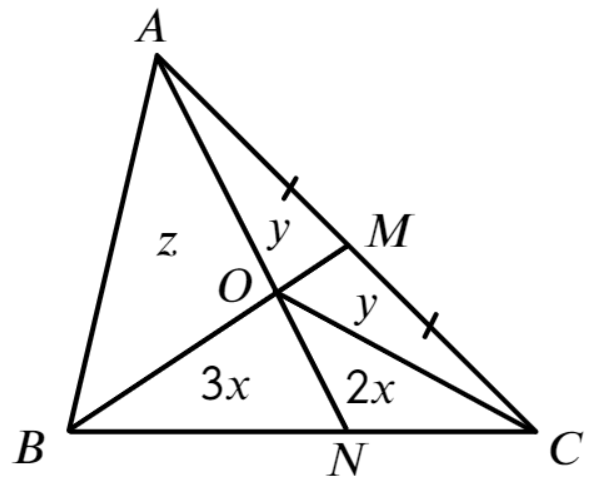
\includegraphics[scale=0.35]{g9-156.png}}
\end{figure}\\
Воспользовавшись тем, что площади треугольников, имеющих общую высоту, относятся как основания, на которые она опущена, введём обозначения: $S_{\Delta OBN}=3x,\ S_{\Delta OCN}=2x,\ S_{\Delta AOM}=S_{\Delta COM}=y,\ S_{\Delta AOB}=z.$ Тогда так как $S_{\Delta ABM}=S_{\Delta CBM},$ имеем равенство $z+y=5x+y,$ откуда $z=5x.$ Так как $S_{\Delta ACN}=\cfrac{2}{3}S_{\Delta ABN},$ получим соотношения $(3x+5x)\cdot\cfrac{2}{3}=2y+2x,\ y=\cfrac{5}{3}x.$ Так как $S_{\Delta ABO}=\cfrac{5}{3}S_{\Delta BON},$ получаем $BO:OM=5:3,$ а так как $\cfrac{S_{\Delta ABO}}{S_{\Delta AOM}}=3,$ получаем $BO:OM=3:1.$\\
